\documentclass[parskip=half]{scrarticle}
\usepackage{amsmath}
\usepackage{graphicx}

\title{Lab 2: Combinational Circuits}
\subtitle{CSC258H1 -- Computer Organization}

% TODO: Enter your name
\author{Your Name}

\begin{document}
\maketitle

\section*{Part I}

The 4-to-1 multiplexers I designed using two-level logic, hierarchical design with logic gates, and hierarchical design with CMOS gates are shown in the figure below.

\begin{figure}[ht!]
    \centering
    % 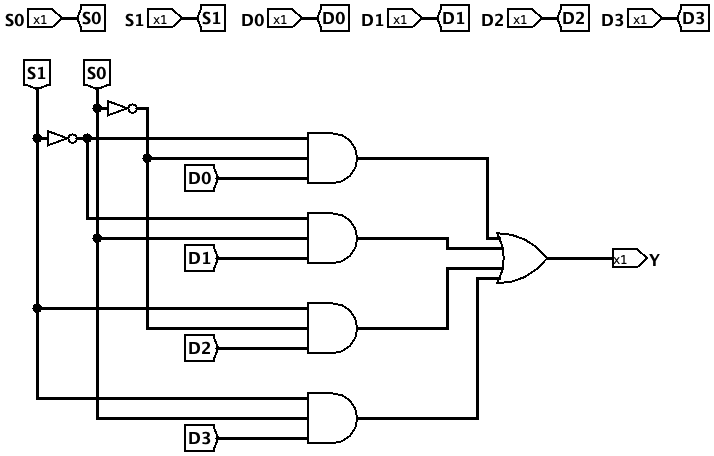
\includegraphics[width=0.7\textwidth]{part1_twolevel.png}
    \caption{A schematic for TwoLevelMux41}
\end{figure}

\begin{figure}[ht!]
    \centering
    % 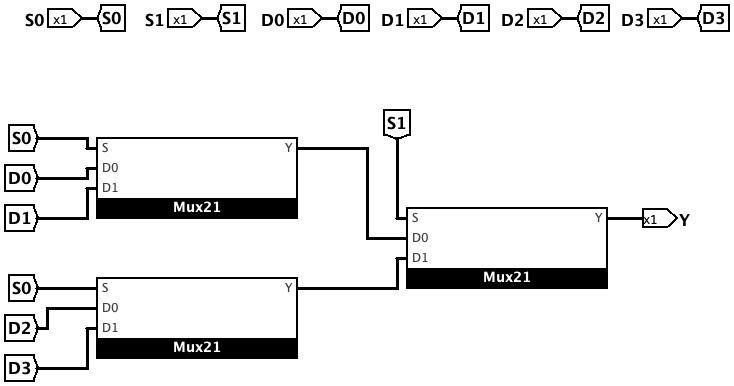
\includegraphics[width=0.7\textwidth]{part1_hierarchical41.png}
    \caption{A schematic for HierarchicalMux41}
\end{figure}

\begin{figure}[ht!]
    \centering
    % 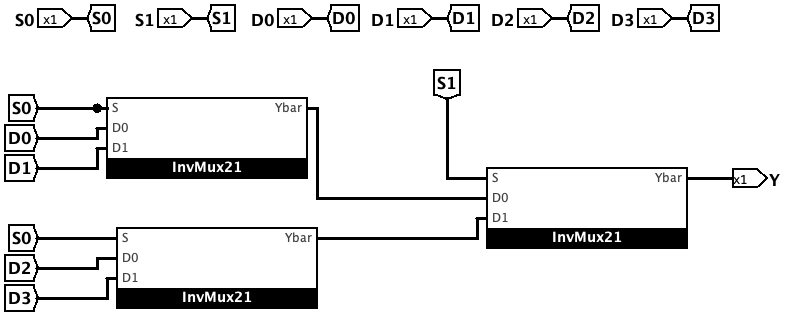
\includegraphics[width=0.7\textwidth]{part1_aoi41.png}
    \caption{A schematic for AOI22Mux41}
\end{figure}

\begin{enumerate}
\item Assume each logic gate is made following the CMOS process.
How many transistors are required for each of your 4-to-1 multiplexer designs?
Show your work by identifying how many transistors are necessary for each gate and sub-circuit used.
% TODO
\end{enumerate}

\section*{Part II}

\begin{enumerate}
\item Derive seven truth tables, one for each segment of the 7-segment decoder.
% TODO

\begin{table}[ht!]
\small
\centering
\begin{tabular}{c|c|ccccccc}
$D_{3:0}$& Character & $S_0$ & $S_1$ & $S_2$ & $S_3$ & $S_4$ & $S_5$ & $S_6$\\
\hline
0000 & 0 \\
0001 & 1\\
0010 & 2\\
0011 & 3\\
0100 & 4\\
0101 & 5\\
0110 & 6\\
0111 & 7\\
1000 & 8\\
1001 & 9\\
1010 & A\\
1011 & b\\
1100 & c\\
1101 & d\\
1110 & E\\
1111 & F\\
\end{tabular}
\end{table}

\item Use Karnaugh maps to write seven Boolean functions for each segment so that they are optimized.
% TODO

\begin{align*}
    S_0 &= ... \\
    S_1 &= ... \\
    S_2 &= ... \\
    S_3 &= ... \\
    S_4 &= ... \\
    S_5 &= ... \\
    S_6 &= ... \\
\end{align*}

\item 
    Export the subcircuit schematic of each segment as an image and include it in your report.
    % TODO

\begin{figure}[ht!]
    \centering
    % 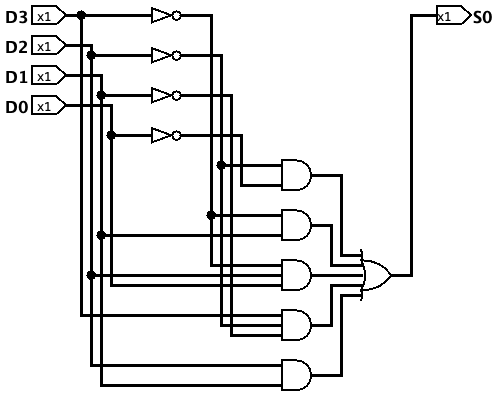
\includegraphics[width=0.7\textwidth]{part2_hex0.png}
    \caption{A schematic of Hex0}
    \label{f:part2_hex0}
\end{figure}

\begin{figure}[ht!]
    \centering
    % 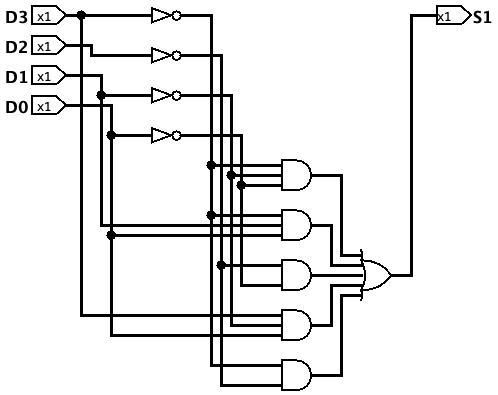
\includegraphics[width=0.7\textwidth]{part2_hex1.png}
    \caption{A schematic of Hex1}
    \label{f:part2_hex1}
\end{figure}

\begin{figure}[ht!]
    \centering
    % 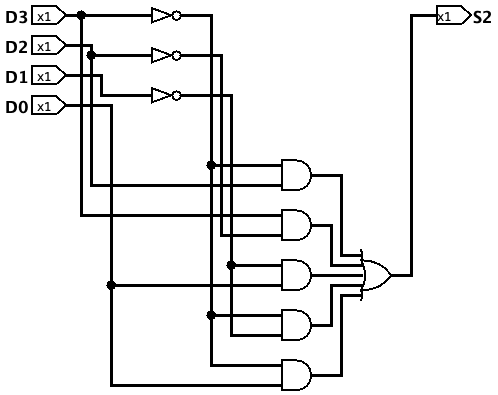
\includegraphics[width=0.7\textwidth]{part2_hex2.png}
    \caption{A schematic of Hex2}
    \label{f:part2_hex2}
\end{figure}

\begin{figure}[ht!]
    \centering
    % 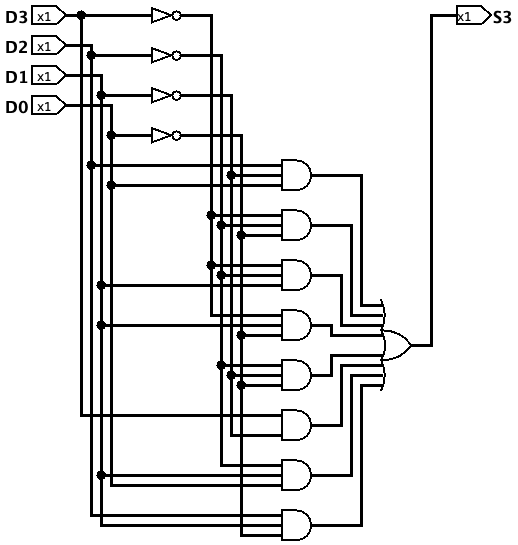
\includegraphics[width=0.7\textwidth]{part2_hex3.png}
    \caption{A schematic of Hex3}
    \label{f:part2_hex3}
\end{figure}

\begin{figure}[ht!]
    \centering
    % 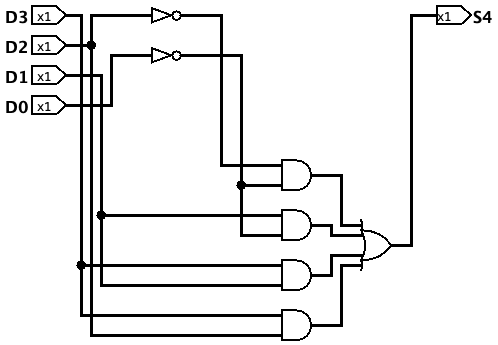
\includegraphics[width=0.7\textwidth]{part2_hex4.png}
    \caption{A schematic of Hex4}
    \label{f:part2_hex4}
\end{figure}

\begin{figure}[ht!]
    \centering
    % 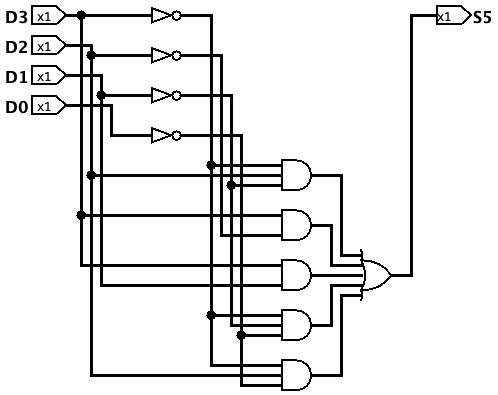
\includegraphics[width=0.7\textwidth]{part2_hex5.png}
    \caption{A schematic of Hex5}
    \label{f:part2_hex5}
\end{figure}

\begin{figure}[ht!]
    \centering
    % 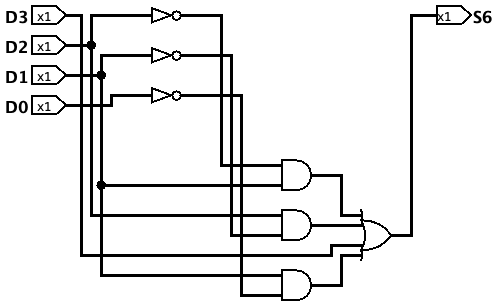
\includegraphics[width=0.7\textwidth]{part2_hex6.png}
    \caption{A schematic of Hex6}
    \label{f:part2_hex6}
\end{figure}
\end{enumerate}

\end{document}